\chapter{Descrierea soluției}

\section{Modurile de funcționare}

În cadrul acestui sistem automat de analiză a jocurilor de tenis de masă se disting următoarele moduri de funcționare, determinate de argumentele primite din linia de comandă:

\begin{itemize}
    \item \textbf{Vedere monoculară} – Se utilizează o singură cameră de înregistrat, plasată în planul lateral.
    \item \textbf{Vedere stereoscopică} – Se utilizează două camere de înregistrat, plasate în planul lateral și orizontal.
\end{itemize}

În plus, este permisă selectarea atât fișierelor video, cât și a directoarelor de imagini ca sursă de intrare pentru procesarea dintr-un singur unghi. Pentru videoclipuri sunt extrase cadrele și procesate, iar pentru directoarele de imagini se iterează prin fiecare element, presupunându-se că imaginile sunt ordonate crescător. În urma procesărilor, cadrele vor fi adunate într-un videoclip în directorul de ieșire, care va avea același nume ca resursa utilizată și va avea fie numărul de cadre pe secundă utilizate de resursa de intrare, fie 60 cadre pe secundă dacă este director de imagini.

\section{Extragerea obiectelor statice}
\label{subsec:static-objects}

O provocare majoră în acest pas o reprezintă integrarea funcţionalităţii în contexte variate, deoarece luminozitatea scenei, tipul suprafeţei de joc şi poziţionarea camerei influenţează considerabil rezultatele. Iniţial, am testat tehnici clasice de vedere artificială filtrare HSV, eroziune şi dilatare\cite{gonzalez1992digital}, însă acestea s-au dovedit prea sensibile la schimbările de fundal. Prin urmare, Algoritmul~\ref{alg:table} prezintă o soluţie bazată pe \textbf{GDINO} şi \textbf{SAM} pentru segmentarea semantică a mesei şi a fileului, ulterior rafinăm masca prin operaţii morfologice de eroziune (\(\ominus\)) şi dilatare (\(\oplus\)), utilizând un kernel K de dimensiune 41×33 pixeli. Fileul, fiind prea îngust pentru a fi detectat direct cu \textbf{GDINO}, este identificat prin diferenţa dintre masca semantică (Figura~\ref{fig:table-sam-2}) şi conturul mesei (Figura~\ref{fig:table-sam-3}), iar centrul acestei regiuni, delimitate de punctele de extrem $\partial \mathbf{P}_{\min}$ și $\partial\mathbf{P}_{\max}$. este apoi transmis către \textbf{SAM} pentru a genera masca finală a fileului. Rezultatul final este ilustrat în Figura \ref{fig:osai-post}.


\begin{algorithm}
\caption{Detectarea și segmentarea mesei și a fileului de tenis.}
\label{alg:table}
\begin{algorithmic}[1]
    \Require Imaginea inițială: \(I_0\)
    \Ensure Măștile segmentate: \(\mathcal{M}_{table}\), \(\mathcal{M}_{net}\)

    \State $p \gets\textit{"table"} $
    \State $K \gets \mathbf 1_{41\times 33}$
    \vspace{0.3em}
    \State
    $M \gets \mathrm{SAM}(I_0, \mathrm{GDINO}(I_0, p))$
    
    \vspace{0.3em}
    \State 
    $M' \gets (M \ominus K)\oplus K$
    \vspace{0.3em}
    
    \State 
    $M_{table} \gets \mathrm{Contur}(M')$
    \vspace{0.3em}

    \State 
      \(P \gets M' \setminus M_{table}\)
    \vspace{0.3em}
    
    \State 
    $\partial P \gets \mathrm{Contur}(P)$
    \State $\mathbf{c} \gets \frac{1}{2} \left( \partial \mathbf{P}_{\min} + \partial\mathbf{P}_{\max} \right)$

    \vspace{0.3em}
    \State 
    $M_{net} \gets \mathrm{SAM}(I_0, c)$
    
\end{algorithmic}
\end{algorithm}


\begin{figure}[H]
    \centering
    
    \begin{subfigure}[b]{0.48\linewidth}
        \centering
        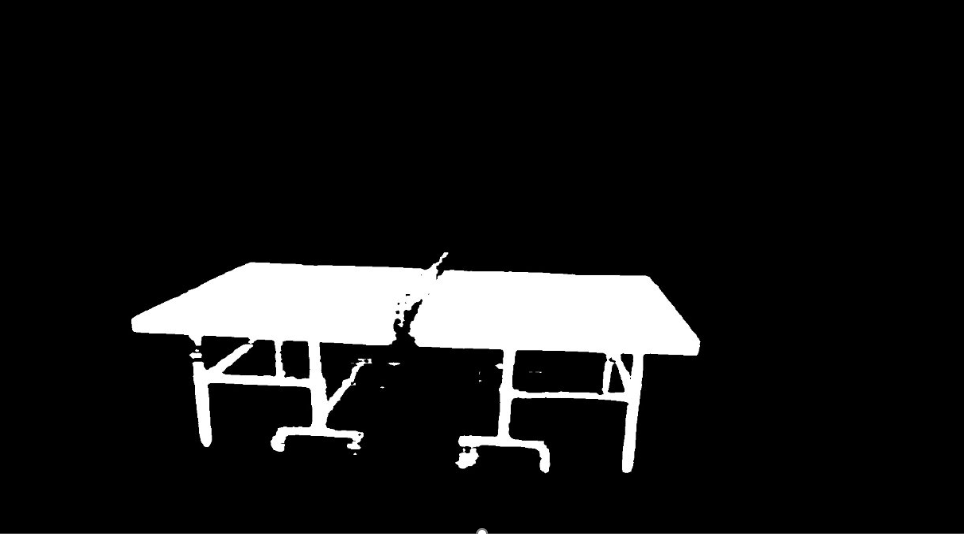
\includegraphics[width=\linewidth]{images/table-sam-1.png}
        \caption{Segmentarea semantică a mesei.}
        \label{fig:table-sam-1}
    \end{subfigure}
    \hfill
    \begin{subfigure}[b]{0.48\linewidth}
        \centering
        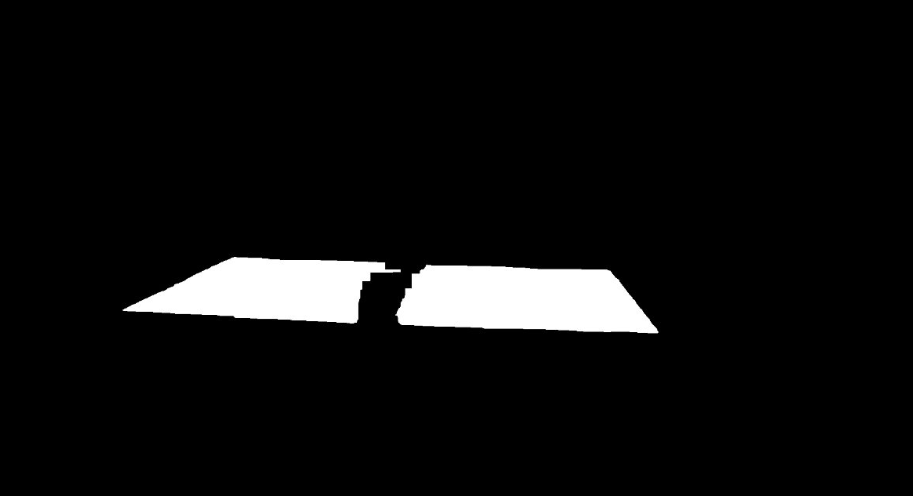
\includegraphics[width=\linewidth]{images/table-sam-2.png}
        \caption{Filtrarea zgomotului.}
        \label{fig:table-sam-2}
    \end{subfigure}
    
    \vspace{0.5cm}
    
    \begin{subfigure}[b]{0.48\linewidth}
        \centering
        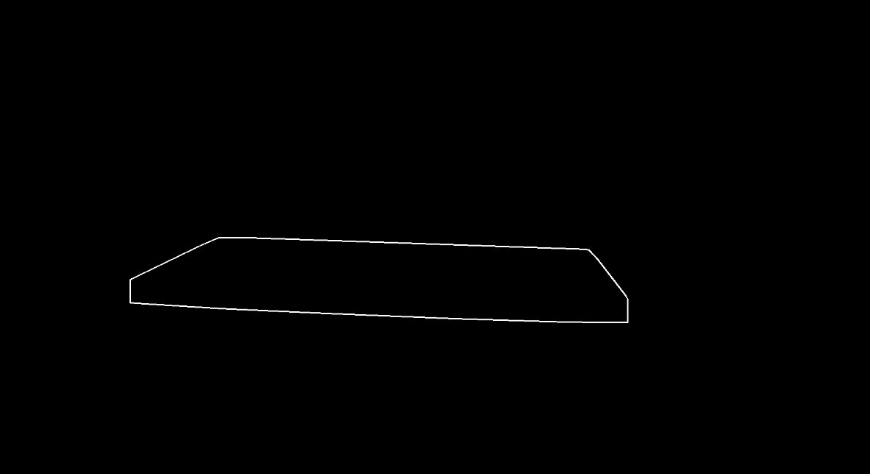
\includegraphics[width=\linewidth]{table-sam-3.png}
        \caption{Extragerea conturului mesei.}
        \label{fig:table-sam-3}
    \end{subfigure}
    \hfill
    \begin{subfigure}[b]{0.48\linewidth}
        \centering
        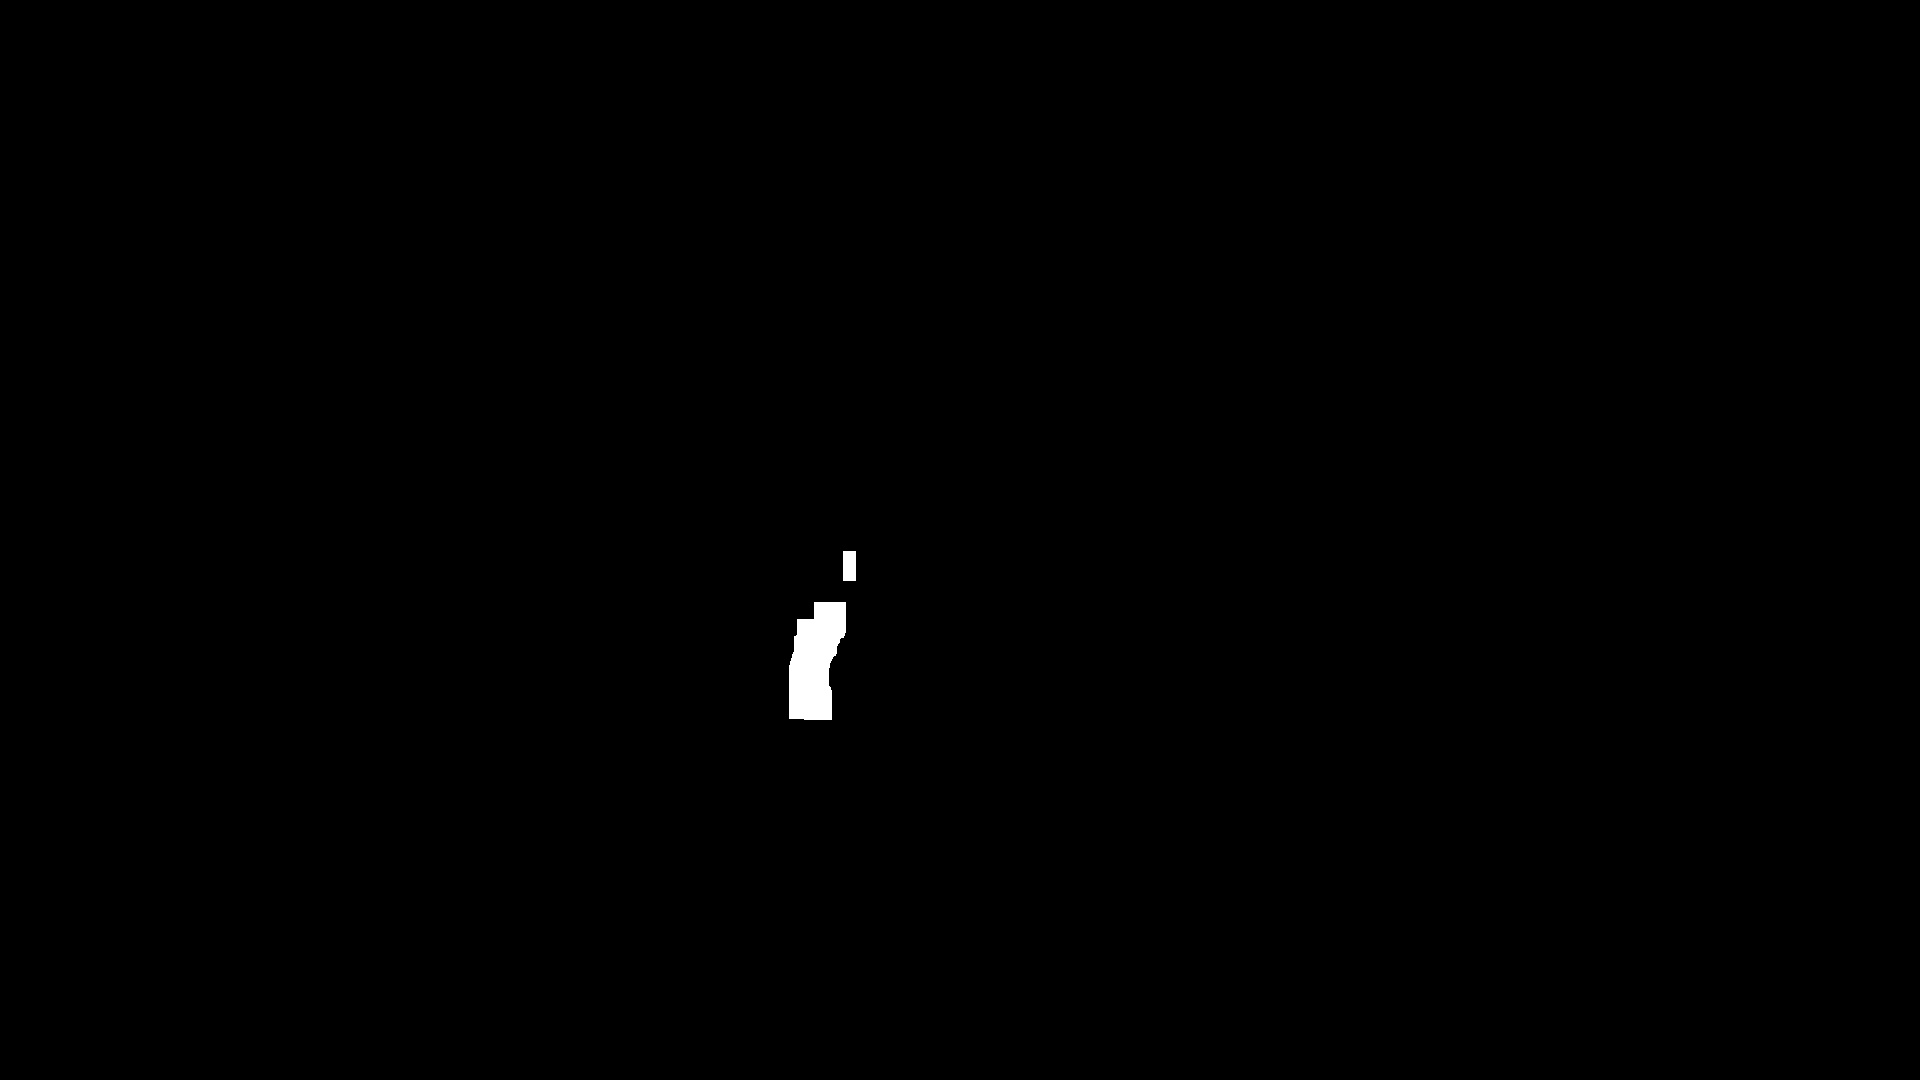
\includegraphics[width=\linewidth]{images/table-sam-4.png}
        \caption{Extragerea inițială a fileului.}
        \label{fig:table-sam-4}
    \end{subfigure}
    
    \vspace{0.5cm}
    
    \begin{subfigure}[b]{0.48\linewidth}
        \centering
        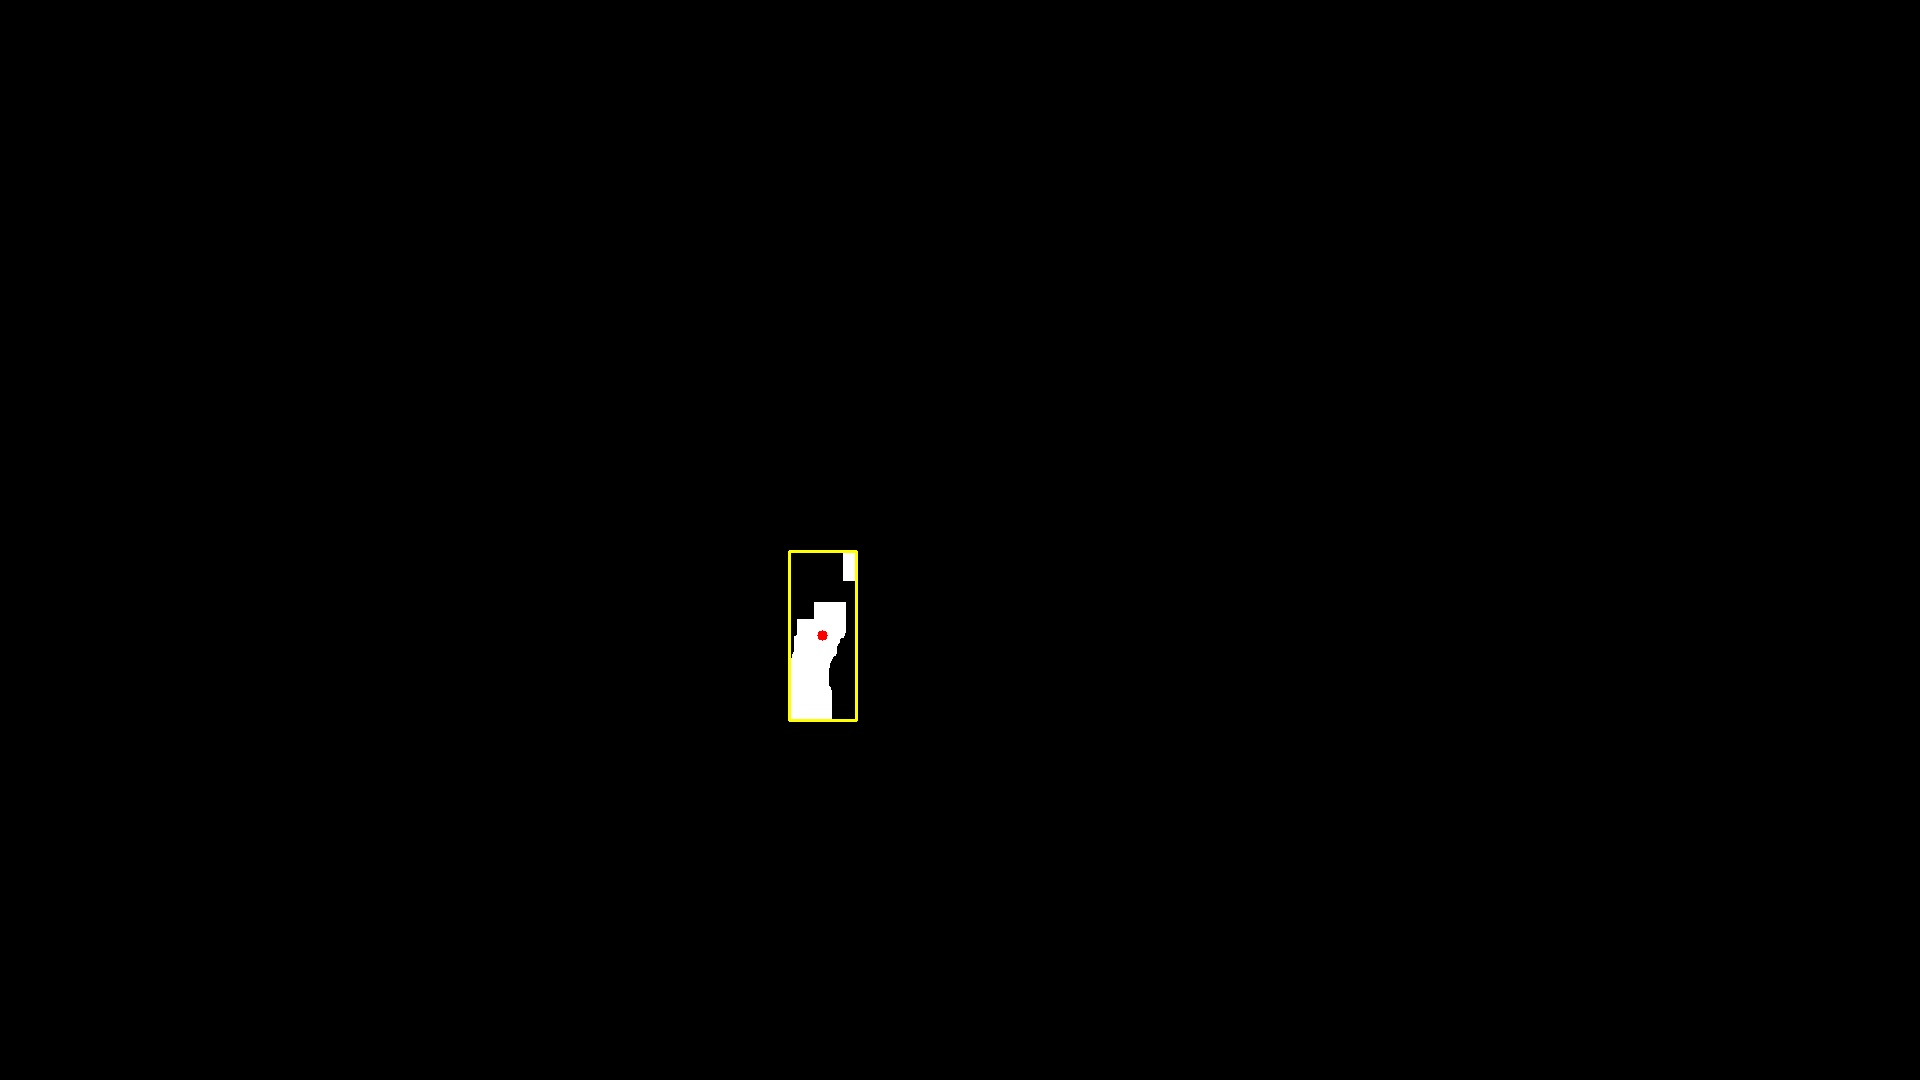
\includegraphics[width=\linewidth]{images/table-sam-5.png}
        \caption{Fereastra de încadrare a fileului.}
        \label{fig:table-sam-5}
    \end{subfigure}
    \hfill
    \begin{subfigure}[b]{0.48\linewidth}
        \centering
        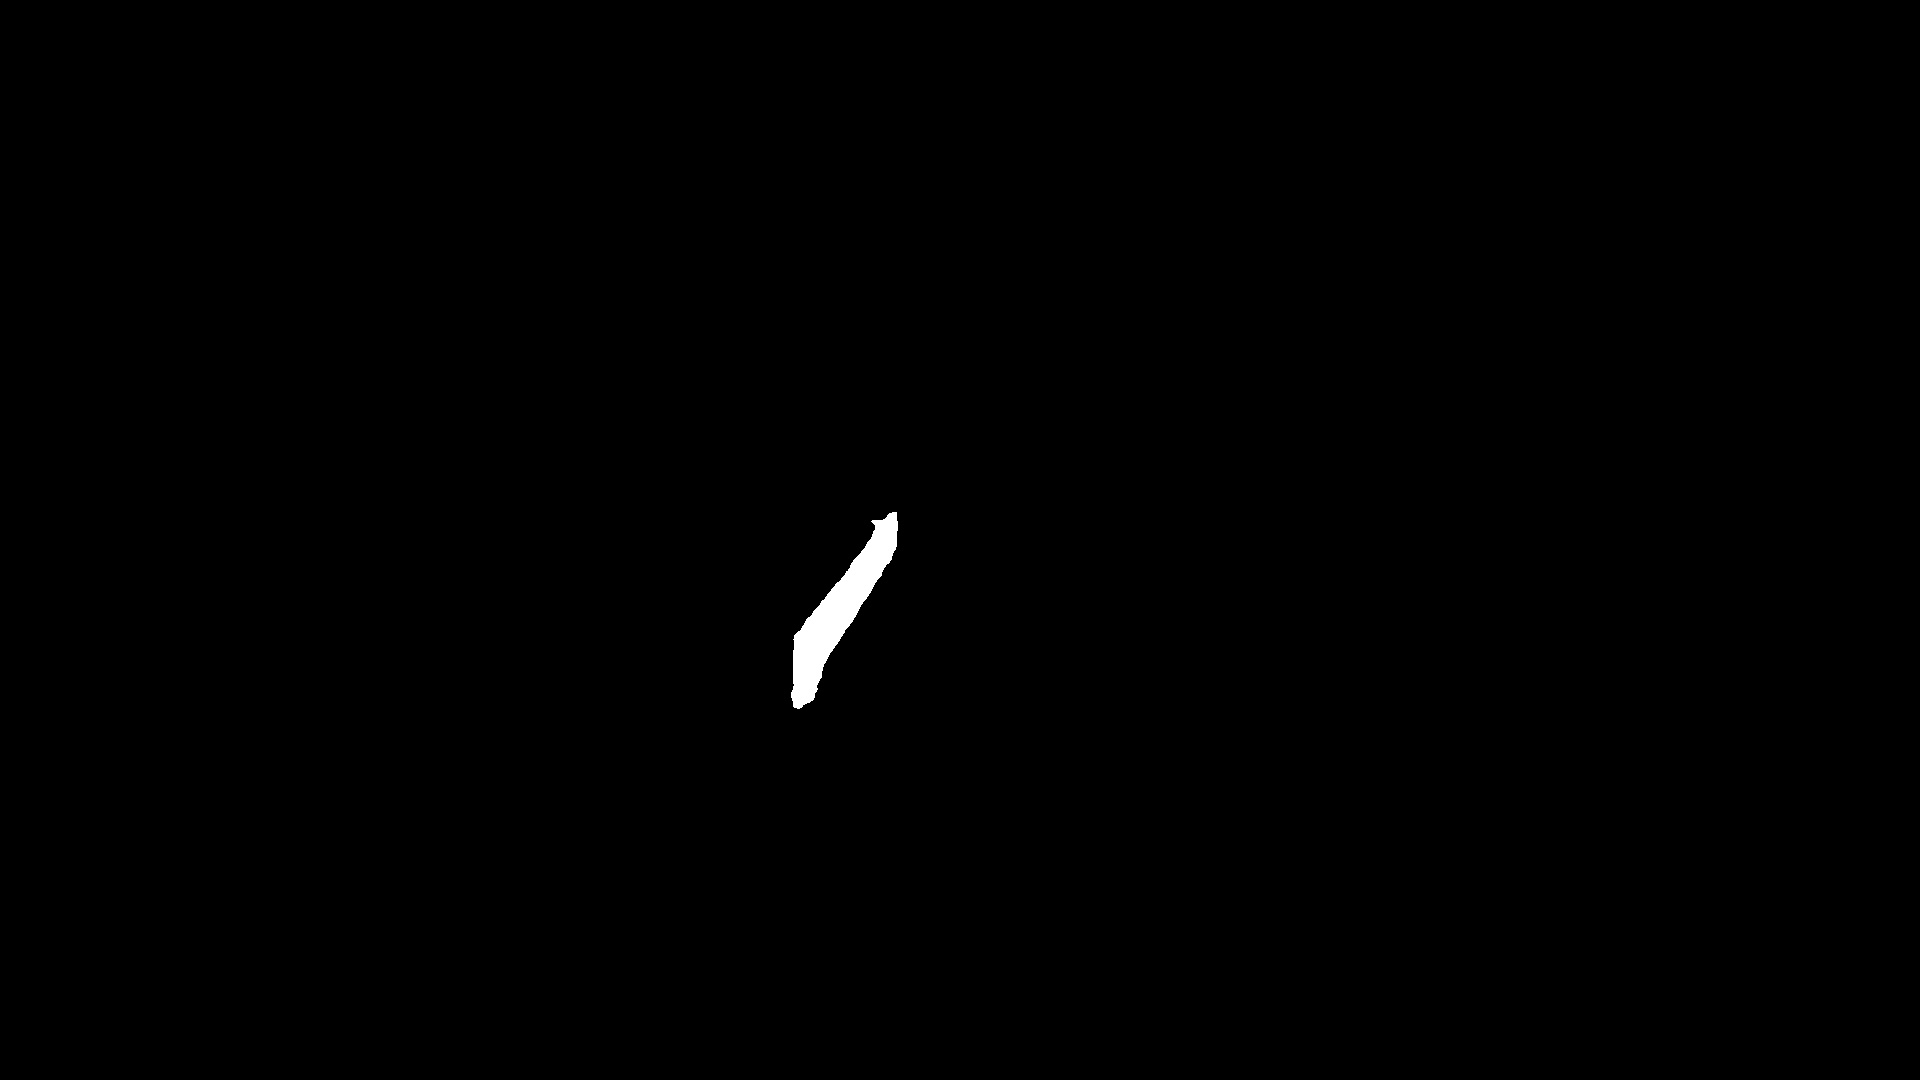
\includegraphics[width=\linewidth]{images/table-sam-6.png}
        \caption{Masca finală obținută pentru fileu.}
        \label{fig:table-sam-6}
    \end{subfigure}
    
    \caption{Etapele detectării mesei de tenis.}
    \label{fig:table-sam}
\end{figure}

% \begin{figure}[H]
%     \centering
%     \begin{subfigure}[b]{0.45\linewidth}
%         \centering
%         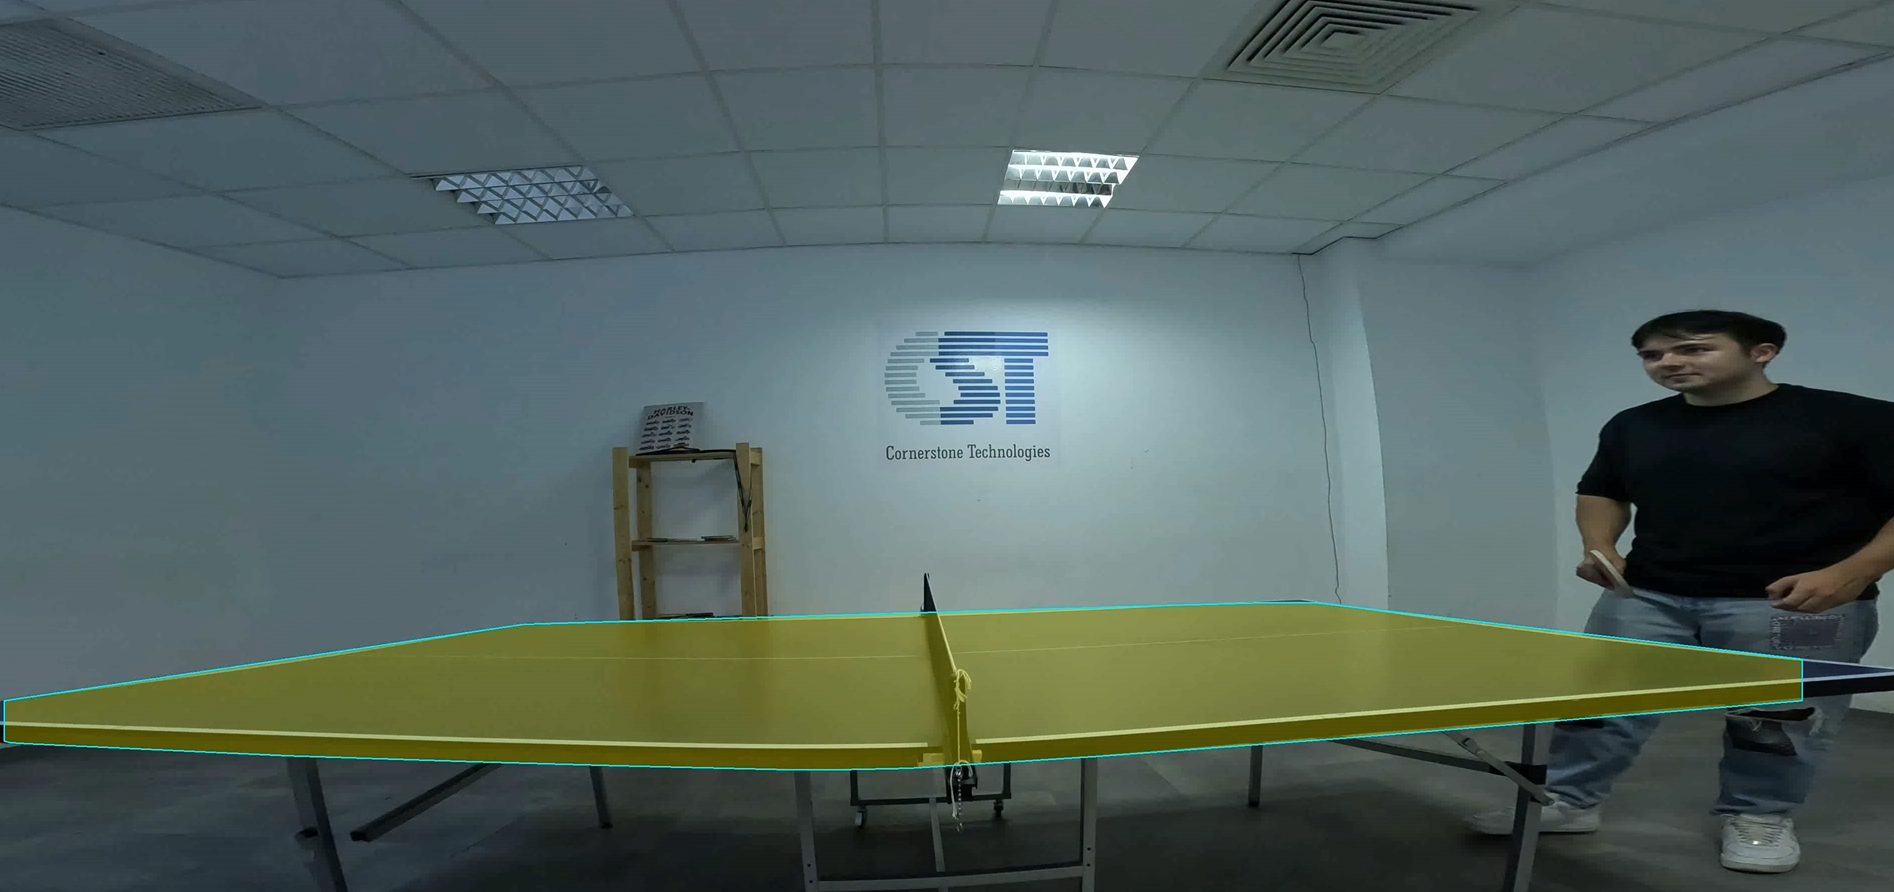
\includegraphics[width=\linewidth]{images/table-sam-results-2.png}
%         \caption{Rezultatul final}
%         \label{fig:table-sam-results-2}
%     \end{subfigure}
%     \hfill
%     \begin{subfigure}[b]{0.45\linewidth}
%         \centering
%         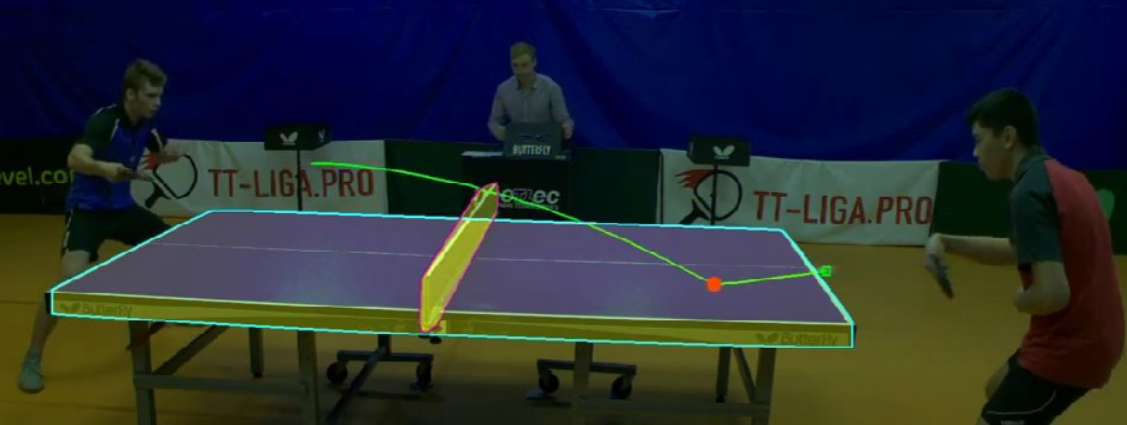
\includegraphics[width=\linewidth]{table-sam-result.png}
%         \caption{Rezultatul final OSAI}
%         \label{fig:table-sam-result}
%     \end{subfigure}
%     \caption{Compararea rezultatelor finale}
% \end{figure}


\section{Extragerea obiectelor dinamice}
\label{subsec:dynamic-objects}
Pentru extragerea elementelor dinamice, mingea si paletele de tenis de masă, vom adapta un model preantrenat YOLO, astfel încât să poată detecta pentru fiecare cadru posibile poziții ale obiectelor de interes. O alternativă inițială pentru detectarea elementelor dinamice a fost cea de potrivire a tiparelor în care cu ajutorul unui set de forme alese manual decidem ce obiect clasificăm, am renunțat la această abordare deoarece introducea multe detecții fals pozitive.

În alegerea versiunii YOLO, am considerat două criterii: un număr cât mai redus de parametri și un nivel al acurateței detecțiilor care să îndeplinească cerințele finale. În urma testelor, YOLOv5 s-a dovedit a fi cea mai potrivită alegere, oferind o acuratețe adecvată obiectivelor proiectului, cu un număr de parametri cu 20\% mai mic decât YOLOv12n și aproximativ 40\% mai mic decât YOLOv8n.

\begin{table}[h]
    \centering
    \begin{tabular}{lcccccc}
        \toprule
        Model & Dimensiune (px) & mAPval 50-95 & Parametri (M) \\
        \midrule
        YOLOv12n \cite{yolov12} & 640 & 40.4 & 2.5 \\
        YOLOv8n \cite{yolov8} & 640 & 37.3 & 3.2 \\
        YOLOv5n-seg \cite{yolov5} & 640 & 27.6 & 2.0 \\
    \end{tabular}
    \caption{Compararea modelelor YOLO.}
    \label{tab:yolo_comparison}
\end{table}

\subsection{Extragerea paletelor de tenis de masă}
\label{subsec:paddle-detect}
În privința paletelor, imaginile $\{I_t\}_{t=1}^{T}$ sunt introduse în modelul YOLO pentru a obține lista detecțiilor $\{D_t\}_{t=1}^T$, iar în funcție de poziția centrului detecției, $\mathrm{xc}(b_i)$, față de centrul imaginii, $\tfrac{\mathrm{width}(I_t)}{2}$, sunt clasificate în paleta jucătorului din stânga, $\{{p^\ell}_t\}_{t=1}^T$, și paleta jucătorului din dreapta, $\{p^{r}_t\}_{t=1}^T$, unde vom selecta detecția cu scor maxim, procesul fiind descris în Algoritm~\ref{alg:paddle-detection}.

\begin{algorithm}[H]
\caption{Detecția paletelor de tenis de masă.}
\label{alg:paddle-detection}
\begin{algorithmic}[1]
\Require Secvență de imagini: $\{I_t\}_{t=1}^{T}$
\Ensure Pozițiile paletelor: $\{p^{\ell}_t\}_{t=1}^T$, $\{p^{r}_t\}_{t=1}^T$
\For{$t = 1$ \textbf{to} $T$}
    \State $D_t \gets \mathrm{YOLO}(I_t)$         \Comment{$D_t = \{(b_i, s_i)\}_{i=1}^{n_t}$}
    \vspace{0.5em}
    \State $L_t \gets \{(b_i,s_i)\in D_t \mid \mathrm{xc}(b_i) < \tfrac{\mathrm{width}(I_t)}{2}\}$
    \vspace{0.5em}
    \State $R_t \gets D_t \setminus L_t$
    \vspace{0.5em}
    \State $p^{\ell}_t \gets \displaystyle\arg\max_{(b_i,s_i)\in L_t} s_i$
    \vspace{0.5em}
    \State $p^{r}_t \gets \displaystyle\arg\max_{(b_i,s_i)\in R_t} s_i$
\EndFor
\end{algorithmic}
\end{algorithm}



\subsection{Extragerea mingii de tenis de masă}
\label{subsec:ball-detect}
Extragerea mingii de tenis de masă este o problemă dificilă, în special dacă sursa de lumină și aparatele de înregistrat sunt de o calitate redusă. Mingea este un obiect cu deplasare rapidă, iar identificarea sa intră în categoria obiectelor denumite \textit{Fast Moving Objects (FMO\cite{Rozumnyi_2017})}, un domeniu dedicat urmăririi și reconstrucției obiectelor care se mișcă cu viteză mare.

Conform teoremei Nyquist\cite{Shannon1949}, pentru a capta și procesa corect un semnal de o anumită frecvență, este necesară achiziția acestuia cu o frecvență cel puțin dublă. Astfel, într-un scenariu de interior iluminat cu surse de lumină fluorescentă, unde frecvența curentului în Europa este de 50 Hz, este necesară utilizarea unei camere cu o frecvență de filmare de cel puțin 100 Hz. În caz contrar, pot apărea distorsiuni semnificative ale obiectelor care se deplasează rapid.

Acest efect poate fi observat în exemplul din Figura~\ref{fig:outside}, unde mingea este clar vizibilă, comparativ cu scenariul Figura~\ref{fig:inside}, unde mingea apare distorsionată din cauza interferențelor cu iluminarea artificială.

\begin{figure}[H]
    \centering
    
    \begin{subfigure}[b]{0.45\linewidth}
        \centering
        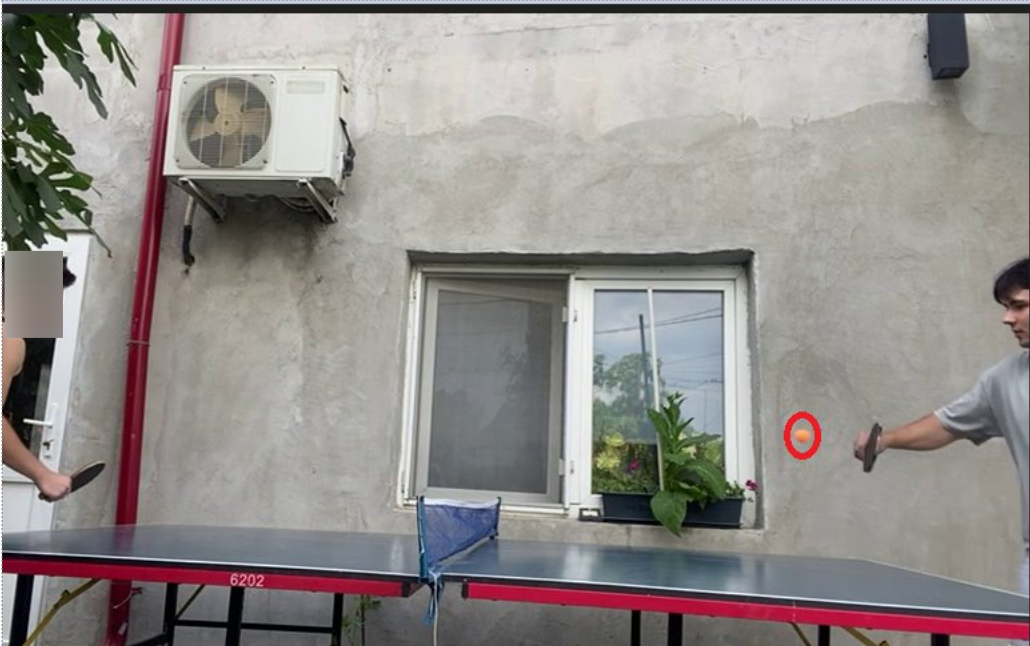
\includegraphics[width=\linewidth]{images/outside.png}
        \caption{Cadru surprins în lumină naturală.}
        \label{fig:outside}
    \end{subfigure}
    \hfill
    \begin{subfigure}[b]{0.45\linewidth}
        \centering
        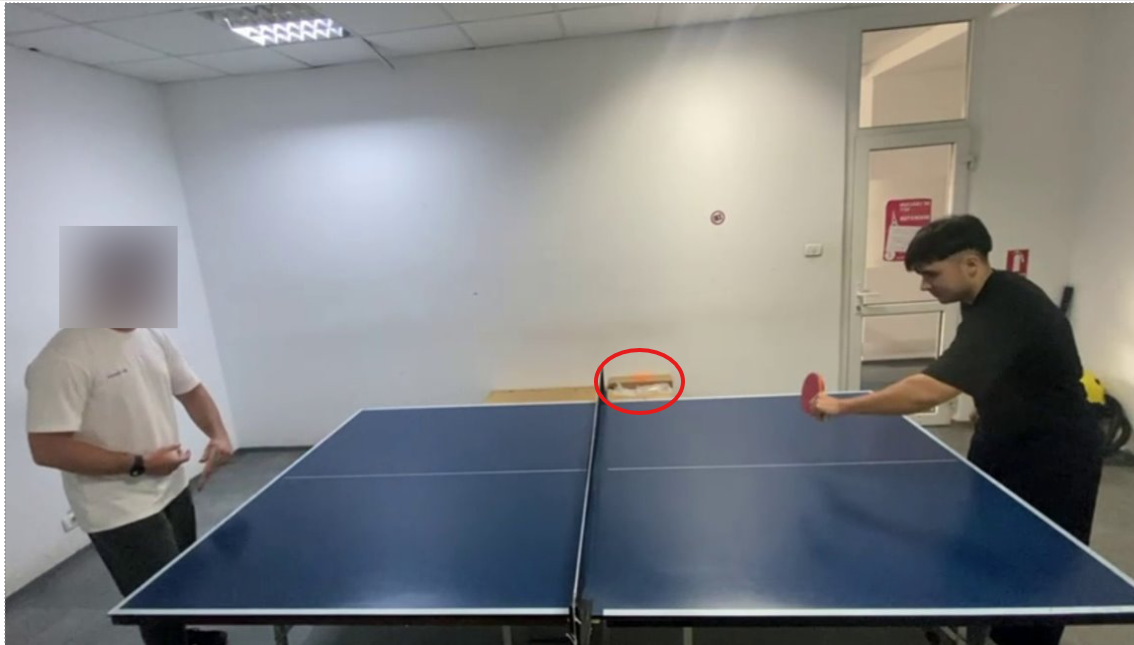
\includegraphics[width=\linewidth]{images/inside.png}
        \caption{Cadru surprins in lumină artificială.}
        \label{fig:inside}
    \end{subfigure}

    \caption{Influența sursei de lumină asupra cadrelor.}
    \label{fig:outside-inside}
\end{figure}

Algoritm~\ref{alg:ball} parcurge seria de imagini $\{I_t\}_{t=1}^T$ și returnează secvența de pozițiile  mingii $\{p_t\}_{t=1}^T$. La pasul $t$, se calculează $D_t=\{(b_i,s_i)\}_{i=1}^{n_t}$, unde $b_i=\{x_i,y_i,w_i,h_i\}$ este fereastra de încadrare a detecției $i$, și $s_i\in[0,1]$ este scorul de încredere, ulterior fiind ajustat în $s_i^{\mathrm{adj}}$ în funcție de poziția precedentă a mingii, iar pentru primul cadru procesat inițializăm cu scorul oferit de YOLO.


\begin{algorithm}[H]
\caption{Detecția mingii de tenis de masă.}
\label{alg:ball}
\begin{algorithmic}[1]
\Require Secvență de imagini: $\{I_t\}_{t=1}^{T}$
\Ensure Lista pozițiilor mingii de tenis de masă: $\{p_t\}_{t=1}^T$
\For{$t = 1$ \textbf{to} $T$}
    \State $D_t \gets \mathrm{YOLO}(I_t)$ 
    \Comment{$D_t = \{(b_i, s_i)\}_{i=1}^{n_t}$}
    \If{$t = 1$}
        \State $i^* \gets \displaystyle\arg\max_{i} s_i$
        \State $p_t \gets b_{i^*}$
    \Else
        \ForAll{$(b_i,s_i)\in D_t$}
            \State $c_i \gets \mathrm{center}(b_i)$
            \State $d_i \gets \|c_i - center(p_{t-1})\|$
            \State $s_i^{\mathrm{adj}} \gets s_i - (d_i/w_{I_t}) $
        \EndFor
        \State $i^* \gets \displaystyle\arg\max_{i} s_i^{\mathrm{adj}}$
        \State $p_t \gets b_{i^*}$
    \EndIf
\EndFor
\end{algorithmic}
\end{algorithm}

\section{Detectarea evenimentelor din tenisul de masă}
În tenisul de masă, identificăm două tipuri de evenimente semnificative: contactul mingii cu masa, care înseamnă o modificare de direcție pe axa \( O_y \), respectiv loviturile de retur ale mingii, care apar atunci când un jucător lovește mingea, determinând o schimbare a direcției pe axa \( O_x \).

\subsection{Detecția contactului mingii cu masa de tenis}
\label{subsec:bounce}
Problema detecției contactului mingii cu masa se reduce la identificarea unor tipare specifice pe baza traiectoriei deja înregistrate la cadrul \( N \). Astfel, vom extrage coordonatele \( O_y \) și ordonându-le în funcție de timp, vom aplica o operație de convoluție (Ec.~\eqref{eq:convolutie}) utilizând un kernel, \(K \gets [-1{.}5,\ 3{.}0, -1{.}5]\). Acest proces este ilustrat în Figura~\ref{fig:convolutie}, unde poziția mingii este tratată ca un semnal unidimensional. Iar prin aplicarea kernelului și utilizarea unui prag de detecție egal cu 0, putem identifica acele puncte din semnal care corespund unui tipar în formă de literă $V$. Mai mult de atât, este verificată intersecția punctului cu conturul mesei.

\begin{equation}
(f \ast g_N)[n] = \sum_{m=0}^{N-1} f[m] \cdot g_N[n-m],
\label{eq:convolutie}
\end{equation}

\begin{algorithm}
\caption{Detecția contactului mingii cu masa de tenis.}
\label{alg:bounce}
\begin{algorithmic}[1]
\Require Lista pozițiilor mingii: $\{(x_i, y_i)\}_{i=1}^N$
\Require Conturul mesei: $\mathcal{T} = \text{Poligon}((x_1, y_1), \dots, (x_n, y_n))$
\Ensure Lista punctelor de contact cu masa de tenis, $S = \{(x_s, y_s)\}_{s=1}^S$

\State $S \gets \emptyset $
\State $K \gets [-1{.}5,\ 3{.}0,-1{.}5]$

\State $D \gets y_{i=1}^N \ast K$ 

\State 
$I = \{i \mid \mathcal{D}_i > 0\}$

\ForAll{$i \in I$}
    \If{$(x_i, y_i) \in \mathcal{T}$}
        \State $\mathcal{S} \gets \mathcal{S} \cup \{(x_i, y_i)\}$
    \EndIf
\EndFor

\end{algorithmic}
\end{algorithm}



\begin{figure}[H]
    \centering
    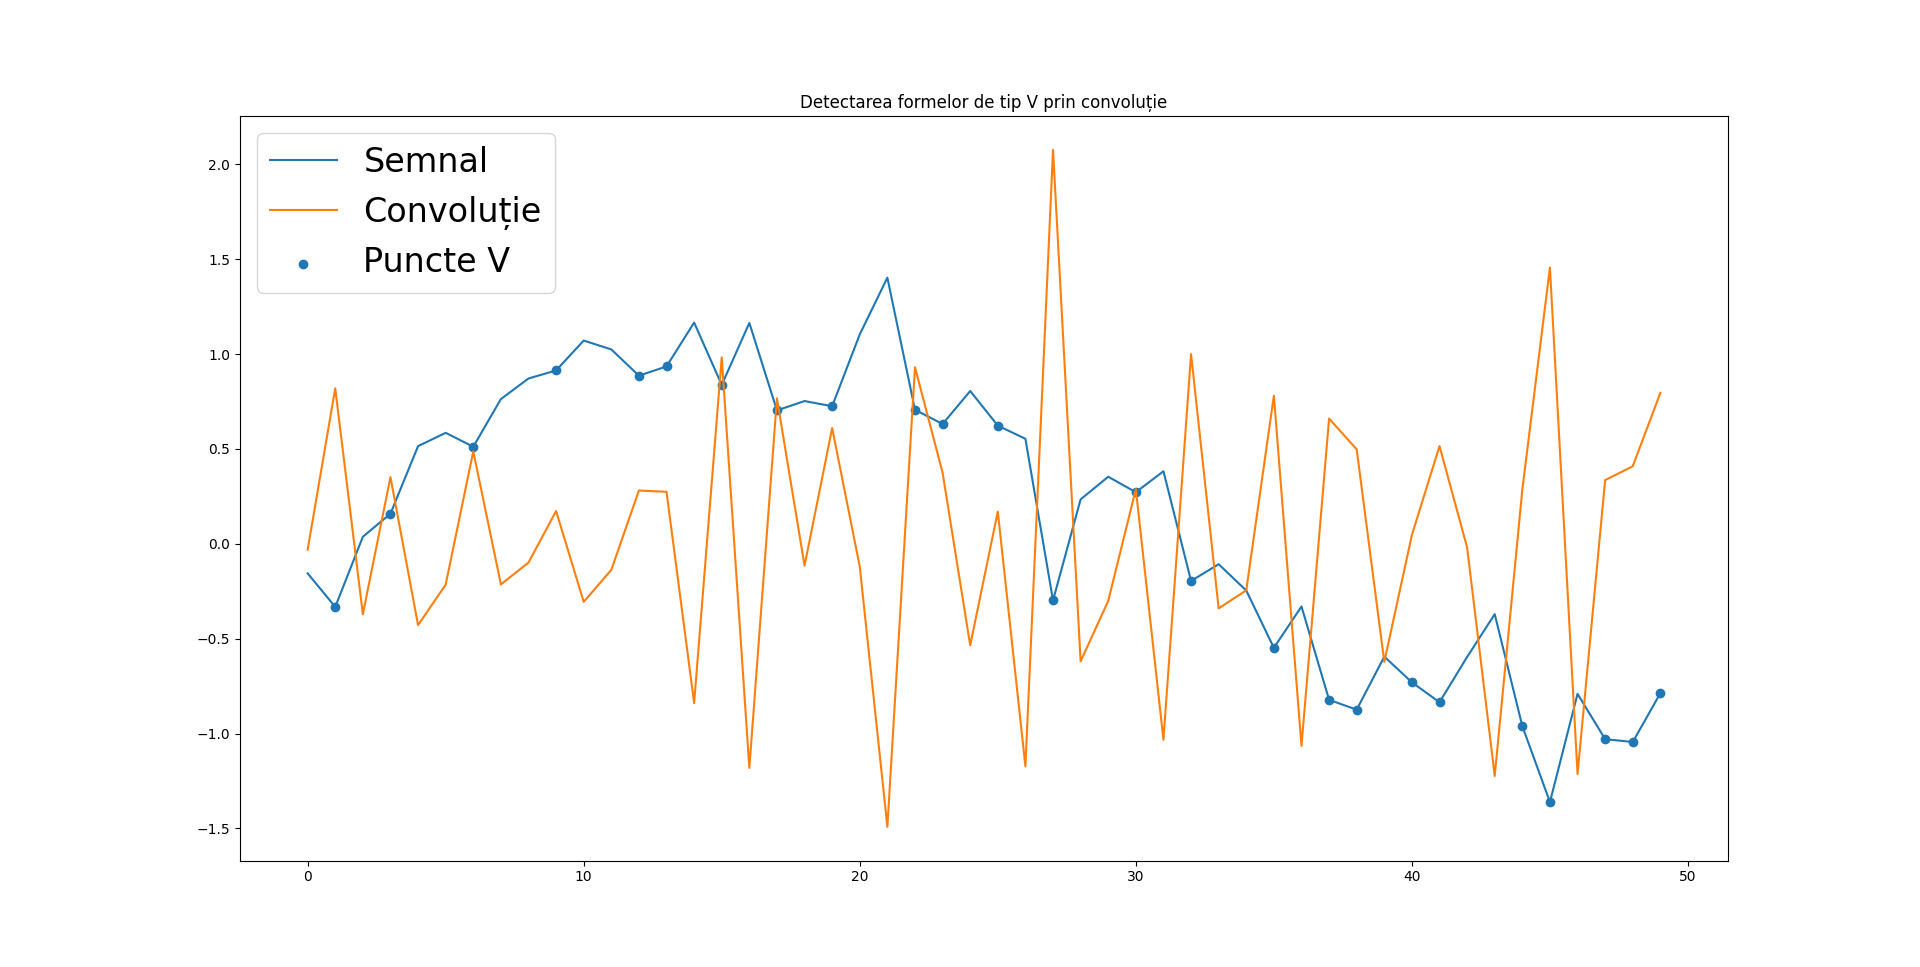
\includegraphics[width=0.8\linewidth]{images/convolutie.png}
    \caption{Aplicarea convoluției pentru a detecta vârfurile $V$.}
    \label{fig:convolutie}
\end{figure}

\subsection{Detecția loviturilor de retur a mingii}
\label{subsec:retur}
Abordarea detecției loviturilor mingii este similară cu cea descrisă în Secțiunea \ref{subsec:bounce}, diferența fiind că de această dată operația este aplicată asupra coordonatei \( O_x \) în loc de \( O_y \) și este verificată intersecția cu conturul unei palete.


\section{Paralelizarea componentelor}

În cadrul acestui proiect vom implementa o arhitectură de tip Producător-Consumator, utilizată frecvent în problemele de concurență, care constă în separarea acțiunilor în a produce sau a consuma pachetul de date. Dificultatea acestei soluții constă în nevoia de a procesa cadrele consecutiv, deoarece pentru fiecare cadru este nevoie de cele \textbf{N-1} cadre precedente pentru a calcula indicatorii. Astfel, folosind procesele explicate anterior, vom introduce o repartizare a acțiunilor pe diferite fire de execuție.

Producătorul va itera prin cadrele resursei, pe care le va transmite către modelul YOLO, procesarea acestora fiind realizată de GPU, eliberând astfel GIL-ul (Global Interpreter Lock) și permițând utilizarea acestuia de către alte fire de execuție. În urma fiecărei procesări, producătorul obține detecțiile claselor de obiecte, aplicând ulterior Algoritm \ref{alg:ball-transition}, Algoritm \ref{alg:paddle-detection}, Algoritm \ref{alg:ball}, Algoritm \ref{alg:bounce} descriși în sectiunile \ref{subsec:paddle-detect}, \ref{subsec:ball-detect}, \ref{subsec:bounce}, \ref{subsec:retur}. Ulterior, după aplicarea algoritmilor, transmitem către Consumator acțiunile care trebuie aplicate asupra cadrelor.
 
Consumatorul verifică dacă există acțiuni de aplicat, iar dacă ele există, va prelua accesul la GIL și va executa instrucțiunile de scriere ale cadrelor pentru a produce videoclipul final. Astfel, paralelizarea se bazează pe operațiunile îndelungate de I/O care pot fi intercalate.

Mai mult decât atât, deoarece rularea modelelor se realizează pe GPU, putem introduce mai multe imagini simultan. Conform mai multor experimente, 32 de imagini reprezintă pragul optim de performanță.

În urma acestor modificări, am observat o creștere semnificativă de \textbf{157\%} în viteza procesării, trecând de la \textbf{14 FPS} la \textbf{36 FPS}. Performanța a fost monitorizată pe același hardware, folosind media a zece procesări consecutive, înainte și după modificări.


\section{Vedere stereoscopică}
În cazul în care este selectat modul de funcționare stereoscopic, este necesară selectarea unui director de fișiere în care sunt prezente două videoclipuri cu denumirile \texttt{upper.mp4} și \texttt{lower.mp4}. Videoclipurile trebuie pornite aproximativ simultan, astfel încât o sincronizare ulterioară a acestora, bazată pe sunet, să fie posibilă. Ulterior, după sincronizare, sunt aplicați aceiași algoritmi de detecție și analiză a jocurilor de tenis de masă, iar coordonatelele sunt reconstruite într-un spațiu tridimensional.

\subsection{Sincronizarea videoclipurilor}
În Figura~\ref{fig:sunet-comparatie} putem observa sincronizarea celor două videoclipuri bazată pe sunet și pe momentele în care mingea atinge masa, acestea având secțiuni cu o amplitudine ridicată.

\begin{equation}
R_{xy}(\tau)=\sum_{n=0}^{N-1} x[n]\;y[n+\tau],
\label{eq:crosscorr}
\end{equation}

În Algoritm~\ref{alg:sound} extragem primele cinci secunde de audio din fiecare clip, $V_{\mathrm{lower}}$ și $V_{\mathrm{upper}}$, calculăm corelația încrucișată R (Ec.~\eqref{eq:crosscorr}) și găsim deplasarea \(\tau^\ast\) pentru care aceasta atinge valoarea maximă. Ulterior, în funcție de semnul lui \(\tau^\ast\), deplasăm unul dintre videoclipuri astfel încât cele două să fie sincronizate.

\begin{algorithm}[H]
\caption{Sincronizarea a două videoclipuri pe baza audio.} 
\label{alg:sound}
\begin{algorithmic}[1]
\Require Videoclipuri: $V_{\text{lower}},\; V_{\text{upper}}$
\Ensure  Videoclipuri sincronizate: $V_{\text{lower}}',\; V_{\text{upper}}'$

\State $a_{\text{lower}} \gets \texttt{audio}(V_{\text{lower}}, 5)$
\State $a_{\text{uppper}}  \gets \texttt{audio}(V_{\text{upper}}, 5)$
\State $R \gets \texttt{crossCorrelation}(a_{\text{lower}}, a_{\text{uppper}})$
\State $\tau^\ast \gets \texttt{argMax}(R)$           

\If{$\tau^\ast > 0$}
    \State $V_{\text{upper}}' \gets \texttt{shift}(V_{\text{upper}},\;\tau^\ast)$
    \State $V_{\text{lower}}' \gets V_{\text{lower}}$
\Else
    \State $V_{\text{lower}}' \gets \texttt{shift}(V_{\text{lower}},\;-\tau^\ast)$
    \State $V_{\text{upper}}' \gets V_{\text{upper}}$
\EndIf
\end{algorithmic}
\end{algorithm}



\begin{figure}[H]
    \centering

    \begin{subfigure}[b]{0.45\linewidth}
        \centering
        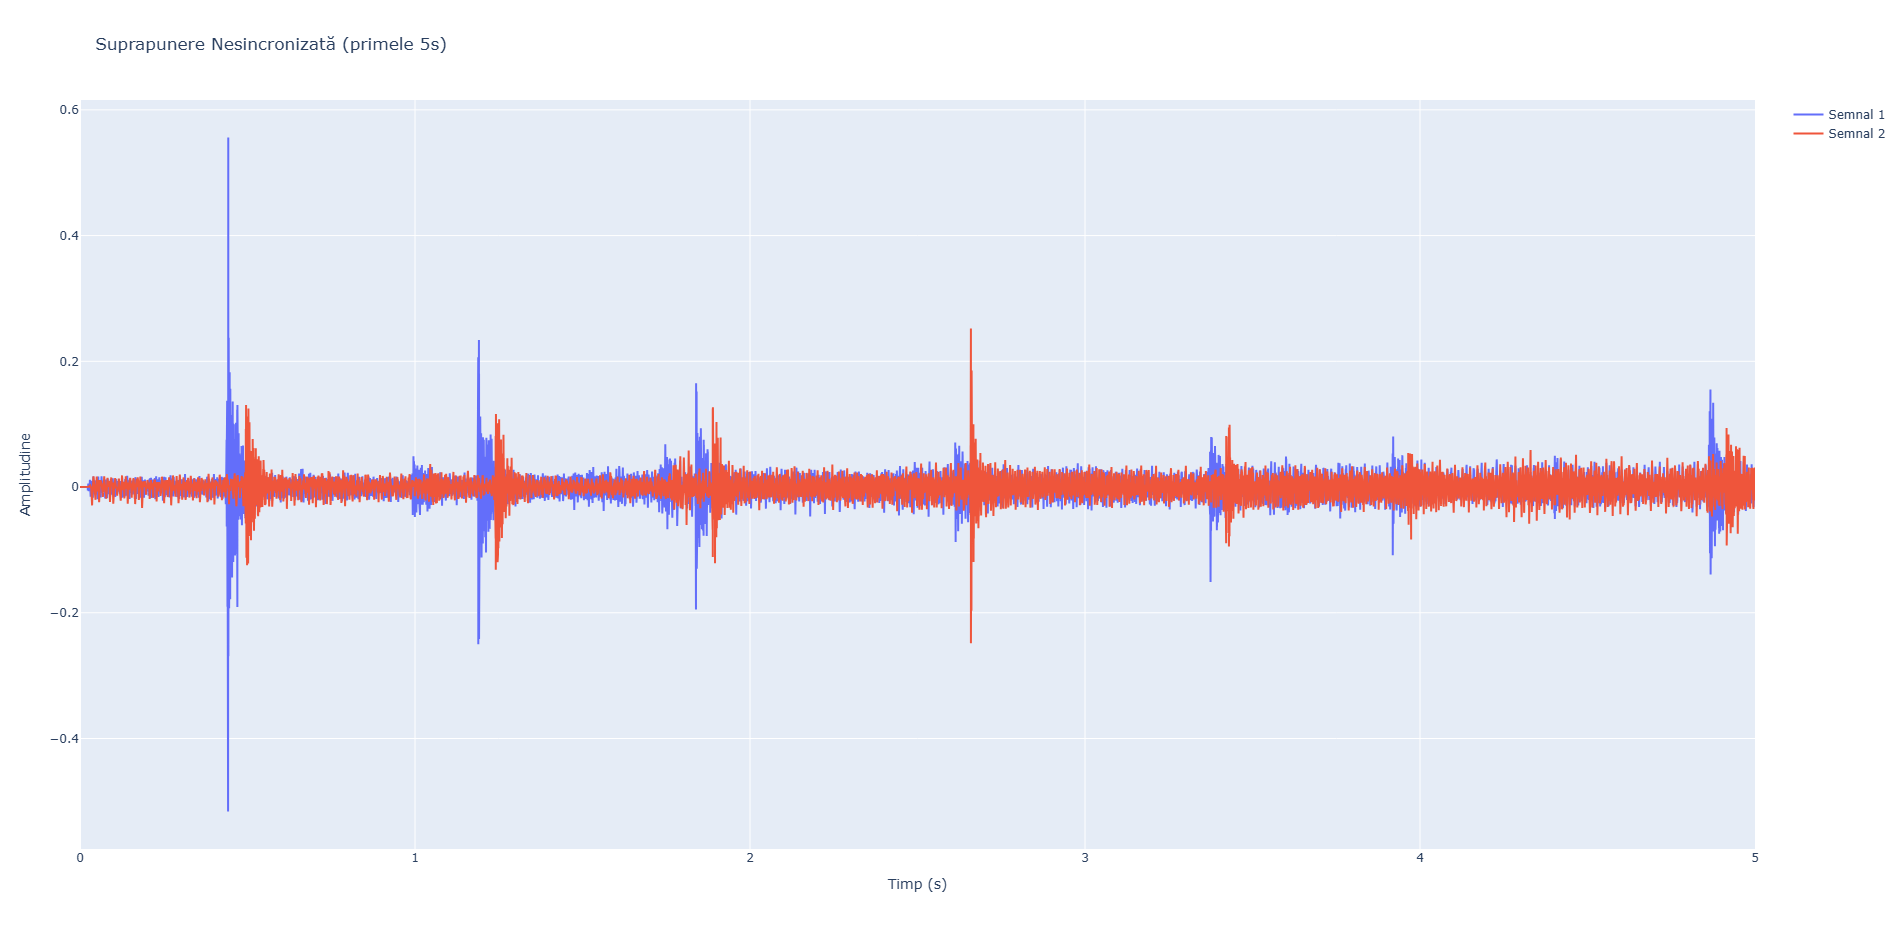
\includegraphics[width=\linewidth]{images/sunet-original.png}
        \caption{Videoclipurile nesincronizate.}
        \label{fig:sunet-original}
    \end{subfigure}
    \hfill
    \begin{subfigure}[b]{0.45\linewidth}
        \centering
        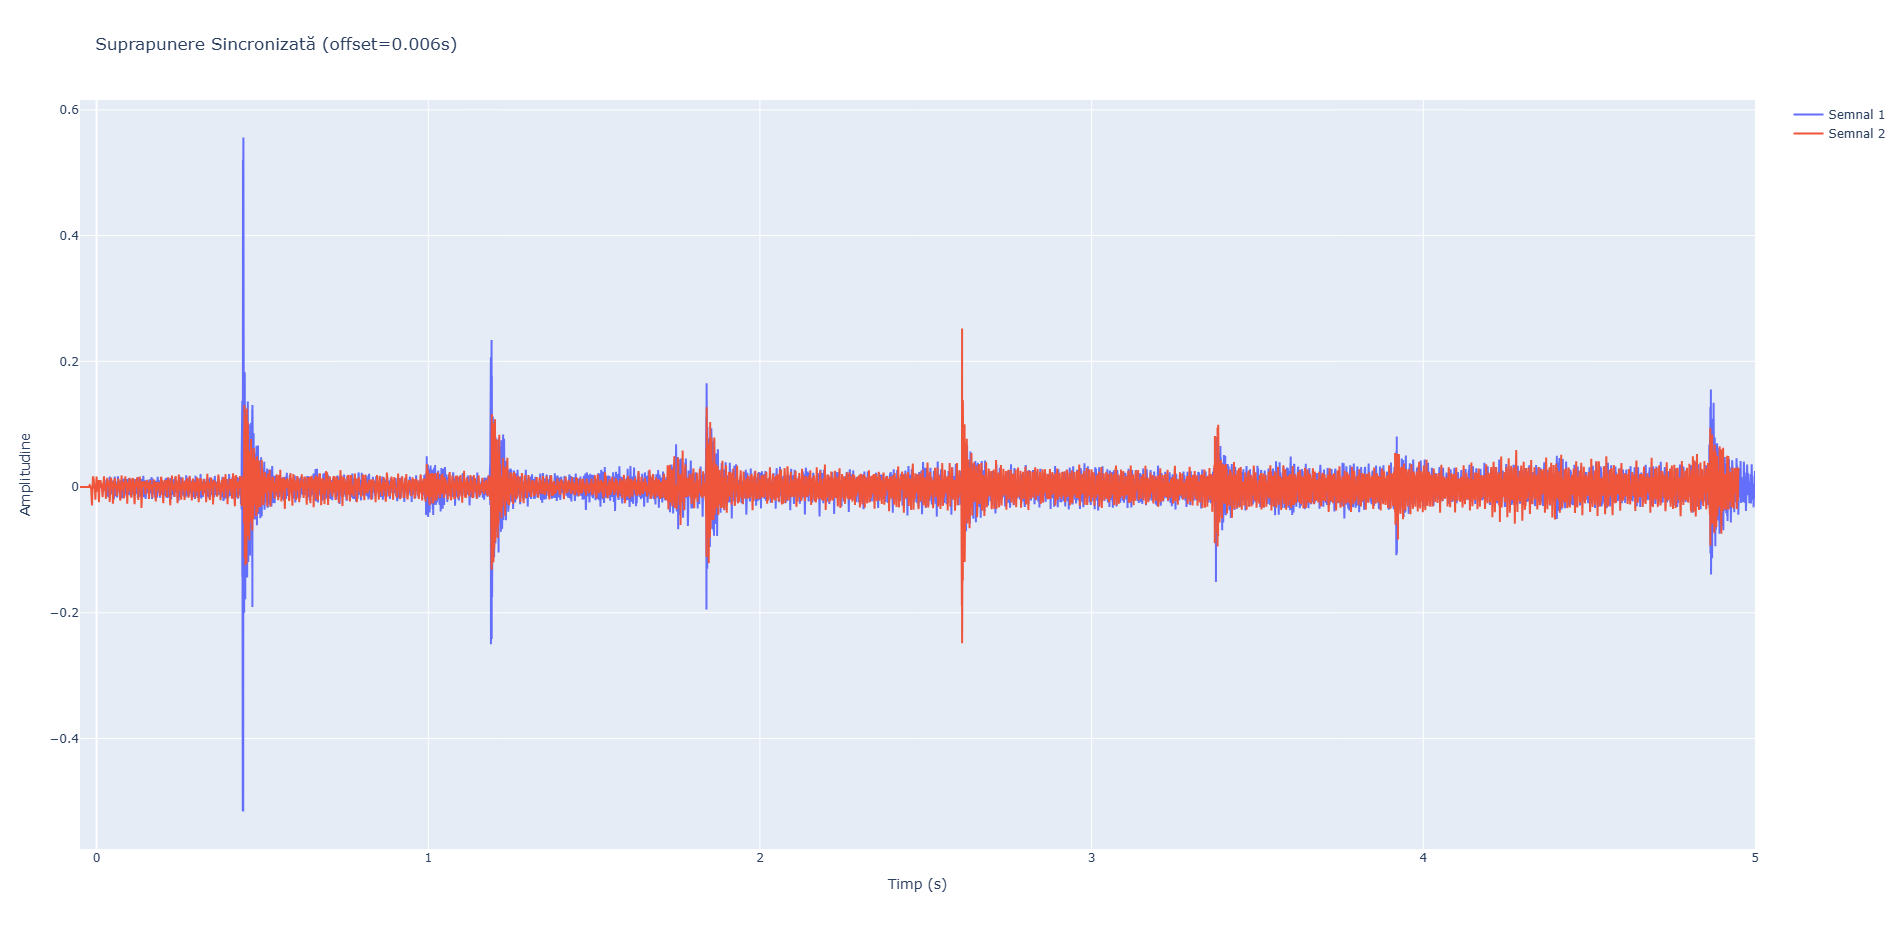
\includegraphics[width=\linewidth]{images/sunet-sincronizat.png}
        \caption{Videoclipurile sincronizate.}
        \label{fig:sunet-sincronizat}
    \end{subfigure}

    \caption{Comparație între sunetul nesincronizat și cel sincronizat.}
    \label{fig:sunet-comparatie}
\end{figure}

\subsection{Construirea coordonatelor 3D}

În urma procesării videoclipurilor sincronizate $V_{\text{lower}}^\prime$ și $V_{\text{upper}}^\prime$, obținem două seturi de coordonate 2D ale mingii de forma $((x_t, y_t), t)$, unde $t$ reprezintă indicele cadrului. Această structură ne permite să unificăm cele două liste de coordonate rezultate din fiecare unghi de filmare și să reconstruim traiectoria mingii într-un spațiu tridimensional.

În Algoritmul~\ref{alg:3d} iniţializăm lista \(\mathcal{P}_{3D}\) ca listă vidă, apoi, pentru fiecare cadru sincronizat, copiem coordonatele \((x,y)\) din videoclipul filmat de sus, iar adâncimea \(z\) o calculăm din videoclipul filmat de jos scăzând poziţia verticală a mingii din înălţimea cadrului, mutând astfel originea sistemului în colţul stânga-jos. Punctul \((x,y,z)\) rezultat este adăugat la traiectorie, iar operaţia se repetă până la ultimul cadru. Rezultatul fiind ilustrat în Figura~\ref{fig:coordonate-comparatie}.

\begin{algorithm}[H]
\caption{Reconstrucția traiectoriei 3D a mingii.}
\label{alg:3d}
\begin{algorithmic}[1]
\Require Seturile de coordonate 2D ale mingii: $\mathcal{P}_\text{upper} = \{(x_i^{\text{upper}}, y_i^{\text{upper}})\}_{i=1}^N$, $\mathcal{P}_\text{lower} = \{(x_i^{\text{lower}}, y_i^{\text{lower}})\}_{i=1}^N$
\Require Înălțimea imaginii videoclipului lateral: $h_{lower}$
\Ensure Setul coordonatelor 3D ale mingii: $\mathcal{P}_{3D} = \{(x_i, y_i, z_i)\}_{i=1}^N$

\State $\mathcal{P}_{3D} \gets \emptyset$
\For{$i = 1$ la $N$}
    \State $x_i \gets x_i^{\text{upper}}$ 
    \State $y_i \gets y_i^{\text{upper}}$
    \State $z_i \gets h_{lower} - y_i^{\text{lower}}$ 
    \State $\mathcal{P}_{3D} \gets \mathcal{P}_{3D} \cup (x_i, y_i, z_i)$
\EndFor
\end{algorithmic}
\end{algorithm}


\begin{figure}[H]
    \centering
    \begin{subfigure}[b]{0.46\linewidth}
        \centering
        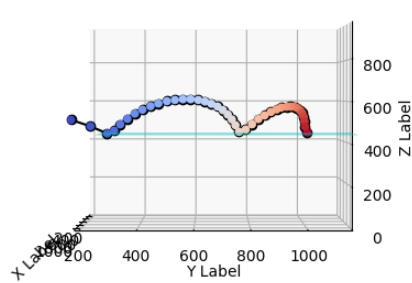
\includegraphics[width=\linewidth]{images/coordonate-1.png}
        \label{fig:coordonate-1}
    \end{subfigure}
    \hfill
    \begin{subfigure}[b]{0.46\linewidth}
        \centering
        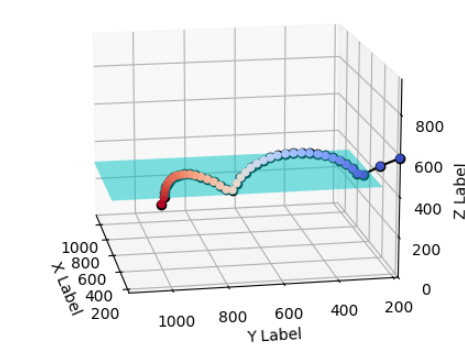
\includegraphics[width=\linewidth]{images/coordonate-2.png}
        \label{fig:coordonate-2}
    \end{subfigure}
    \caption{Coordonatele în spațiu tridimensional.}
    \label{fig:coordonate-comparatie}
\end{figure}

